\documentclass{clgrammar}

\title{kijazu Kunci}
%\subtitle{The Language of Truth}

\author{san Kunci}

\usepackage[backend=biber, style=mla]{biblatex}
\addbibresource{bib.bib}
\usepackage{fontspec}
\setmainfont{LexendDeca}
\usepackage{qtree}
\usepackage{graphicx}
\usepackage{indentfirst} 
\usepackage{longtable}
\usepackage{layout}
\usepackage{gb4e}
%cyrillic font
\newfontfamily\cf{NotoSans}
%kana font
\newfontfamily\kf{Sazanami Gothic}

%start the document (pretty helpful)
\begin{document}
\frontmatter
%\maketitle
\tableofcontents

\mainmatter
\part{Introduction}

\chapter{Goals}
	kijazu Kunci is a thing (ki) that is spoken (jazu) made by and for me (Kunci). It's main goal is to make obscuring one's true intent, accidentally or intentionally, as hard as possible. This was inspired by George Orwell's essay “Politics and the English Language'', where he argues that we misuse language to ``make lies sound truthful and murder respectable, and to give an appearance of solidity to pure wind'' (\cite{english}). 

	It's other goal is to make presenting subjective opinions as objective fact impossible. <more later when i feel like writing it>

%	This philosophy originally comes from the LRI philosophy, which was never written down or fully completed. The LRI philosophy was something along the lines of ``minimalism because get to the point of what you want to say''.
	
\part{Grammar}

\chapter{Phonology}

\section{Consonants}

\begin{center}
    \begin{tabular}{l|c|c|c|c}
                  & Labial & Dental & Palatal & Velar \\
        \hline
		Nasal     &      m & n      &         &      \\
		Plosive   & p,b    & t,d    &         &  k,g \\
		Fricative &        & s,z    & š       &    x  \\
		Affricate &        &  c     & č       & \\
        Tap       &        & r & & \\
		Aprox.    & w &  & j &
    \end{tabular}
\end{center}

\section{Vowels}

\begin{center}
    \begin{tabular}{l|c|c}
        & Front & Back \\
        \hline
        Close & i  & u  \\
        Mid & e  & o  \\
        Open & a 
    \end{tabular}
\end{center}

To ensure that every word is easy and quick to pronounce, each syllable is (C)(j)V(n).

\section{Pitch Accent}

A rising pitch falls on the first syllable in a word. Monosyllabic particles are treated as part of the previous word. This differentiates compound from 2 adjacent words.

\section{Allophony}
An /n/ will become velar before a /k/ or a /g/, and will become /m/ before a /p/ or /b/.

\chapter{Syntax}

The syntax of kijazu Kunci is inspired by RPN; there are 2 types of morphemes: operators, which are verb conjugations and particles and operands, which are nouns or constituents. The operator always proceeds its operands. This is show in the syntax tree below, where each operator is italicised. 

\Tree [.ču\ \textit{wa}\ muka\textit{renai}\ doma\ kosa\textit{i}\ \textit{te} [.ču\ \textit{wa}\ muka\textit{renai} [.ču\ wa\ muka\textit{re} [.ču\ \textit{wa} ču \textit{wa} ] muka \textit{re} ] \textit{nai} ] [.doma\ kosa\textit{i} doma kosa \textit{i} ] \textit{te} ]
\begin{exe}
	\ex
	\gll ču wa mukarenai doma kosai te \\
	2.SG NOM eat.NEG.EV.1 house big LOC \\
	\trans `I was told that you eat in the big house'
\end{exe}

There are two types of operators: preserving and non-preserving operands. Operating on the phrase of a preserving operand will modify its first operand, while if it is a non preserving operator it will operate on the whole phrase. For example, in ``doma kosa-i'', ``i'' is a preserving operand, because if something operates on the whole phrase, it is still modifying ``doma''. However, in ``ču wa muka ta muka-re'', ``re'' is a non-preserving operand because, if an operator operates on the whole phrase, it modifies the whole phrase, instead of just ``ču''. All verb conjugations, except for relative clauses, are non-preserving. Every other operator is preserving.



\chapter{Ejo lanrepn (Forms)}

In some roots, the first vowel can be changed to modify the meaning of the word. There are 3 ``forms'' that a word can have. The positive form, represented with an ``a'', the neutral represented with ``e'', and the negative, represented with an ``i''. The positive is used for things that have a generally good connotation or when there is a lot of something. The negative is used for something that has a generally bad connotation or there is few of something. The neutral from is used for something that is inbetween both extremes. Not every every from is used in every word, and not every word has forms. 

For example, with the root ``k*sa'', the negative form is ``kisari'', and means to be small. The neutral from is ``kesari'', meaning to be average/neutral size. The positive form, ``kasari'' means to be large. 


\chapter{Verbs}

Verbs inflect for the past, present and future tense, and the indicative, subjunctive/irrealis, imperative and interrogative moods. 

Infinitive verbs end in ``-ri'', which is replaced with evidentiality and tense from table \ref{verbs}, or ``-xo'' for the imperative. ``-nai-'' is added for negation, and ``-ka'' is added for the interrogative. 

\begin{center}
	\begin{tabular}{l|c|c|c} \label{verbs}
		Evidentiality        & Past & Present & Future \\
		\hline
		Scientific Consensus & -so  & -su     &  -sju  \\
		Speaker has proof    & -to  & -tu     &  -tju  \\
		Speaker reasons      & -no  & -nu     &  -nju  \\
		Speaker witnessed    & -ro  & -ru     &        \\
		Speaker has been told    & -ra  & -re     &  \\ 
		Speaker believes without proof & -go & -gu & -gju \\ 
		Subjunctive          & -bo  & -bu     &  -bju \\
	\end{tabular}
\end{center}	

These are glossed with ``.EV.0-5'', with 5 being scientific consensus and 0 being personal belief.


This unconventional evidentiality system ensures that the speaker knows how the information they are stating is true, and the listener can be ready to challenge their assertions. It also makes it impossible to state witnessing or being told of a future event (without being using more words). 

The subjunctive is only used in statements like ``if this would happen, then I would do that''. See (section)

Changing a verb into an interrogative changes the evidentiality from the perspective of the speaker to the listener. In a quotation, evidentiality is from the perspective of the person who is being quoted.


\chapter{Aspect}

\subsection{Verb Suffixes}
These are added before the verb conjugation and change the meaning of the verb. 

\begin{center}
	\begin{tabular}{l|c}
		Suffixes & Meaning \\
		\hline
		re & to do again\\
		pa & to make\\
		xa & to become \\
		mi & to use improperly\\
		cu & to use\\
		di & to emit/give\\
		kjen & to be able to \\
	\end{tabular}
\end{center}

For example, pjukanamapamirekjenxari means ``to become able to repeatedly improperly write a dictionary''.


\section{Nouns and Adjectives}
Every word in kijazu Kunci is a noun by default; adjectives are created by adding ``-i'' to a noun. Adverbs are adjectives that apply to a verb instead of a noun. Compound words are created by concatenating two or more nouns, order they would otherwise be in. 

\section{The Verb ``suri''} 

In kijazu Kunci, adjectives are only used to express properties that cannot be proven or measured, such as size, temperature, lengths, masses, and distances. Properties that are subjective judgements, such as goodness, beauty, and more are express as a transitive verb, with the subject being who the property is subjective to and the object being the property. This makes presenting subjective judgements as fact impossible, because it is required to specify who observers the property. Nothing can be ``good'', ``bad'', or ``suck''; just things that one likes or dislikes. Food is not "tasty"; one just likes its taste.

All subjective properties can be reduced to liking or disliking a quality of something, thus, the only required subjective property is ``to like'', ``suri'' and its negation, ``masuri''. Here are examples of ``suri'':

\begin{exe}
	\ex
	\gll ja wa ačiwu muka ču jo jo ta suru. \\
	1.SG NOM taste food 2.SG GEN GEN OBJ like.EV.2\\
	\trans `I like.EV.2 the taste of your food.'
\end{exe}

\begin{exe}
	\ex
	\gll jani wa kumi doma jo ta suru.\\
	1.EX NOM look house GEN OBJ like.EV.2 \\
	\trans `We like the look of the house.'
\end{exe}

\section{The Verb ``ron''}

Since there is no objective ``wrong'' and ``right'', kijazu Kunci uses the word ``ron'' to mean ``to agree with''. While in some contexts, such as mathematics, these can be objective, but since there is no way to confine words to a specific context, these words do not exist. 

\section{Comparisons}

Comparisons are made using the verbs ``ori'', its opposite ``maori'' and ``samari'', which mean more, less, and equal to respectively.

\begin{exe}
	\ex
	\gll kosa ja jo wa kosa ču jo ta otu.\\
	size 1 GEN size 2 NOM GEN ACC more-than.EV.4 \\
	\trans `I have proof that I am bigger than you.'
\end{exe}

\begin{exe}
	\ex
	\gll sona ja jo wa sona ču jo ta maotu.\\
	knowledge 1 GEN NOM knowledge 2 GEN ACC less-than.EV.4 \\
	\trans `I have proof that I am smarter than you.'
\end{exe}

\begin{exe}
	\ex
	\gll sona ja jo wa sona ču jo ta samatu.\\
	knowledge 1 GEN NOM knowledge 2 GEN ACC same.EV.4 \\
	\trans `I have proof that we are equally smart.'
\end{exe}

The last one can use two subjects instead.



\chapter{Particles}

Like the rest of the language, particles are head-final, and proceed the noun phrase(s) that the modify.
\begin{center}
	\begin{tabular}{l|c}
		Particle & Case \\
		\hline
		wa & Nominative \\
		ta & Accusative \\
		jo & Genitive \\
		te & Locative \\
		na & Adessive \\
		ko & Dative/Benifactive \\
		ci & Ablative \\
		po & Instrumental \\
		de & Temporal Locative \\
		da & Temporal Adessive \\
		go & Temporal Dative \\
		co & Conjunction \\
		au & Disjunction \\
		i & Adjective Marker \\

\end{tabular}
\end{center}

\section{``wa'' and ``ta''}
The subject is marked with ``wa'' and ``ta'' marks the object. Swapping the order of the subject and object is allowed, and they can be used multiple times for multiple subjects or objects. These particles are not required, and only exist for clarity, and for swapping the order of a verbs arguments. 

\begin{exe}
	\ex
	\gll san sonai wa san kosai ta kumira \\
	person smart.ADJ NOM person big.ADJ see.PST.EV.1 \\
	\trans `I was told a smart person saw the big person.'
\end{exe}


\section{Genitives with ``jo''}
As opposed to many natural languages, ``jo'' takes on two operands, marking the previous operand as genitive to its previous.

\begin{exe}
	\ex 
	\gll tobarišu sonai ja jo wa pjuka ču jo ta jonju \\
	friend smart.ADJ 1 GEN NOM document 2 GEN ACC have.FUT.3 \\
	\trans `I reason that my smart friend will have your book.' 
\end{exe}

\section{Locations}
``te'' is used to show the location where something happens.  

\begin{exe}
	\ex 
	\gll tobarišu wa juto doma te \\
	friend NOM COP.PRS.EV.4 house LOC \\
	\trans `I have proof that the friend is in the house.' 
\end{exe}
 
``na'' is used to show where something is on, at or near.  

\begin{exe}
	\ex 
	\gll muka wa jutju <table> te   \\
	food NOM COP.FUT.EV.4 table ADE \\
	\trans `I have testable proof that the food is on the table' 
\end{exe}

``ko'' is used to show a location, goal, or recipient. 

\begin{exe}
	\ex 
	\gll ja wa ikuro doma ko \\
	1 NOM go.PST.EV.2 house DAT \\ 
	\trans `I experienced that I went to the house.'
\end{exe}

\begin{exe}
	\ex
	\gll kjo wa muka ta pano ja ko \\
	3 NOM food ACC make.PST.EV.3 1 DAT \\
	\trans `A think she made food for me.'
\end{exe}

\begin{exe}
	\ex
	\gll ču wa ki ja ci suruka? \\
	2 NOM thing 1 ABL like.PRS.EV.1.INT \\
	\trans `Do you like the thing that I gave to you?'
\end{exe}

``ci'' can be used to clear up a grammatical ambiguity: if someone gives you a gift, the gift can be treated either your gift or their gift. In kijazu Kunci, it is the gift \textit{from} them, \textit{to} or \textit{of} you. 

\section{Instrumental with ``po''}
``po'' is used to show what is used or how much time is taken.

\begin{exe}
	\ex
	\gll ja wa ni ta pari kjentju pjuka kosai po \\
	1 NOM 3 ACC do.INF can.FUT.EV.4 book INS \\
	\trans `I have testable proof that I will be able to do it using the book.' 
\end{exe}

\begin{exe}
	\ex
	\gll ja wa ni ta mukari kjensu <1> <hour> po\\
	1 NOM 3 ACC eat.INF can.PRS.EV.4 one hour INS\\
	\trans `It is scientific consensus that I can't eat it in an hour' 
\end{exe}



\section{Times}

The Temporal Locative particle ``de'' is used to show when an event takes place, like English `when'.

\begin{exe}
	\ex
	\gll kjo wa mukaru jačo wa mukuru de \\
	3 NOM eat.PRS.EV.2 1.IN eat TLOC \\
	\trans `It eats wen we eat'
\end{exe}

The Temporal Adessive particle ``da'' is used to show when an event starts.
% this is a bad example
\begin{exe}
	\ex
	\gll ču wa mukarenai doma kosai te <day>ni da \\
	2.SG NOM eat.NEG.EV.1 house.ADJ big LOC day.this TDP \\
	\trans `I was told you eat in the big house starting today'
\end{exe}

The Temporal Dative particle ``go'' is used to the when an event ends, like ``until'' in English.
\begin{exe}
	\ex
	\gll ču wa ni ta sunju <day><next> go \\
	2 NOM 3 ACC like.FUT.EV.3 day-next TDAT \\
	\trans `I reason that you will like it until tomorrow.'
\end{exe}


\section{Conjunction and Disjunction}\label{junction}

The particles wa and ta are used multiple times to express multiple subjects or objects. For two verbs, the verbs roots of the verbs, which are operands, are combined with “co”, then, the conjugation goes after co. The disjunctive particle ``au'' is used in the same way that ``co'' is.

\begin{exe}
	\ex
	\gll tinku riso co kjenri\\
	think reason CON can.INF\\
	\trans `to be able to think and reason'
\end{exe}
\section{Relative Clauses}\label{relative-clauses}

Free relative clauses do not need to be marked. When it is an exact quotation where evidentiality is from the perspective of the quotee, the clause must be marked with quotation marks. The particles ``wa'' and ``ta'' are not used in a relative clause.

\begin{exe}
	\ex
	\gll san Wuka wa ``doma kosaru'' ta jazunju\\
	person Wuka NOM house size.PRS.EV.2 ACC speak.FUT.EV.3\\
	\trans `I predict that Wuka will say: ``He sees that the house is big''. 
\end{exe}

This is also valid and the quotes are not needed. 

\begin{exe}
	\ex
	\gll san Wuka wa ni ta jazunju: doma kosaru \\
	person Wuka NOM house size.PRS.EV.2 ACC speak.FUT.EV.3\\
	\trans `I predict that Wuka will say: ``He sees that the house is big''. 
\end{exe}


Bound relative clauses are formed using the operator ``tje'', which makes a non-preserving operator preserving.

\begin{exe}
	\ex
	\gll ja wa pjuka nama jorutje ta sugu  \\
	1 NOM book name have.PRS.EV.2.PRV ACC like.PRS.EV.0 \\
	\trans `I like books that have a name.'
\end{exe}

\chapter{Positions}

There are 6 words for positions: the 4 cardinal directions, front, and back. The cardinal directions are turned into relative directions with a genitive. Wei and bei can be used temporally to refer to before and after.

\begin{center}
	\begin{tabular}{l|c|c}
		Word & Cardinal & Relative \\ 
		\hline 
		xei  & West     & Left     \\
		čei  & South    & Top \\
		kei  & North    & Bottom \\
		rei  & East     & Right \\
		wei  &          & Front \\
		bei  &          & Back \\
	\end{tabular}
\end{center}

\begin{exe}
	\ex
	\gll ni wa tu čei ja jo te. \\
	3 NOM COP.EV.4 south 1 GEN LOC\\
	\trans `It is below me (on my south).'
\end{exe}

\chapter{Numbers}
Each digit (0-9) is a single syllable. They are combined together like the normal Arabic numerals.
\begin{center}
	\begin{tabular}{l|l}
		Word & Value \\
		\hline
		0 & ni \\
		1 & ru \\
		2 & či \\
		3 & ku \\
		4 & ti \\
		5 & re \\
		6 & ro \\
		7 & se \\
		8 & ko \\
		9 & le \\
		10 & runi \\
		11 & ruru \\
		100 & runini \\
		137 & rukuse \\
	\end{tabular}
\end{center}
These numbers are cardinal by default; ordinals are created with the adjective form.

\begin{exe}
	\ex
	\gll san rukusei wa čire pjuka ta joru\\
	person 137.ORD NOM  25 book ACC have.PRS.EV.5 \\   
	\trans `The 137th person has 25 books.'
\end{exe}


\chapter{Computer Tiers}

\chapter{Pronouns and Proper Nouns}

There are 6 pronouns. They can be reduplicated to form plurals.

\begin{center}
	\begin{tabular}{l|c}
		Person & Word \\
		\hline
		1st & ja \\
		2nd & ču \\ 
		3rd & kjo \\
		1st inclusive & jačo \\
		1st exclusive & jani \\
		Demonstrative & ni \\
		Reciprocal/reflexive & use \\
	\end{tabular}
\end{center}

Proper nouns are formed with a classifier, the type of think that the proper noun is, followed by the proper noun, with the first letter capitalized. In ``jazu Kunci'', jazu is is the classifier and Kunci is the proper noun. When, taking foreign names, it is encouraged translate meaning instead of a phonetic approximation; for example, Cyrillic (kirillica) is not ``lika Kiririca'', but ``lika Kirirosu'', because St. Cyril is ``san Kirirosu''.

	Since names get extremely long, only the first one or two syllables of the proper noun are needed, except for the first time the given noun is introduced. This is called the short form. The short form is often used instead of pronouns. 

	The classifiers for countries and people are not required. 

\part{Orthography}

\chapter{Punctuation}
Kijazu Kunci uses 4 punctuation marks: the colon, semicolon, period, and comma. The comma is to show that everything before the comma has been moved from the back of the sentence to the front. The period ends a sentence. The semicolon goes between two operands for additional clarity. The colon is used at the end of a sentence to show that the following sentence explains and unknown in the previous sentence. 

Punctuation can be used in every script, however, it is mostly used while writing in the Roman alphabet, and punctuation is often not used in Vimsonjo.

\chapter{Vimsonjo}
Vimsonjo is a logography that comes from sitelen Pona. It was originally designed for use in LRI. There are 22 radicals in vimsonjo. Each radical is named in toki Pona. Rotated forms exist for all radicals, however, only forms that are used are shown.

\begin{center}
	\begin{longtable}{l|cccccc}
		Name & Default & Soto & Anpa & Sewi & Teje \\
		\hline
		jan & 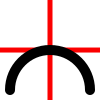
\includegraphics[width=1cm]{images/radicals/jan.png} & 
\includegraphics[width=1cm]{images/radicals/jansoto.png} & 
\includegraphics[width=1cm]{images/radicals/jananpa.png} & 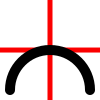
\includegraphics[width=1cm]{images/radicals/jansewi.png} & 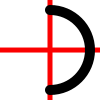
\includegraphics[width=1cm]{images/radicals/janteje.png}  & \\
		luka & 
\includegraphics[width=1cm]{images/radicals/luka.png}& & & &\\ 
		lawa & 
\includegraphics[width=1cm]{images/radicals/lawa.png}& & & &\\ 
		en & 
\includegraphics[width=1cm]{images/radicals/en.png}& & & & &\\ 
		ala & 
\includegraphics[width=1cm]{images/radicals/ala.png}& & & &\\ 
		uta & 
\includegraphics[width=1cm]{images/radicals/uta.png} & & 
\includegraphics[width=1cm]{images/radicals/uta.png} & & 
\includegraphics[width=1cm]{images/radicals/utateje.png} \\ 
		kama & 
\includegraphics[width=1cm]{images/radicals/kama.png} & 
\includegraphics[width=1cm]{images/radicals/kama.png} & 
\includegraphics[width=1cm]{images/radicals/kamaanpa.png} & 
\includegraphics[width=1cm]{images/radicals/kamasewi.png} & 
\includegraphics[width=1cm]{images/radicals/kamateje.png} \\ 
		linja & 
\includegraphics[width=1cm]{images/radicals/linja.png} & & & 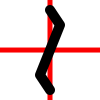
\includegraphics[width=1cm]{images/radicals/linjasewi.png} & \\ 
		palisa & 
\includegraphics[width=1cm]{images/radicals/supa.png} & & & 
\includegraphics[width=1cm]{images/radicals/palisasewi.png} &\\ 
		sike & 
\includegraphics[width=1cm]{images/radicals/sike.png}& & & & \\ 
		poki & 
\includegraphics[width=1cm]{images/radicals/poki.png}& 
\includegraphics[width=1cm]{images/radicals/pokisoto.png} & 
\includegraphics[width=1cm]{images/radicals/pokianpa.png} & 
\includegraphics[width=1cm]{images/radicals/pokisewi.png} & 
\includegraphics[width=1cm]{images/radicals/pokiteje.png} \\ 
		kule & 
\includegraphics[width=1cm]{images/radicals/kule.png}& & & & \\ 
		weka & 
\includegraphics[width=1cm]{images/radicals/weka.png}& & & & \\ 
		soweli & 
\includegraphics[width=1cm]{images/radicals/soweli.png}& & & &\\ 
		nasin & 
\includegraphics[width=1cm]{images/radicals/nasin.png}& & & &\\ 
		tenpo & 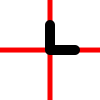
\includegraphics[width=1cm]{images/radicals/tenpo.png}& & & &\\ 
		pana & 
\includegraphics[width=1cm]{images/radicals/pana.png}& & & &\\ 
		noka & 
\includegraphics[width=1cm]{images/radicals/noka.png}& & & &\\ 
		lili & 
\includegraphics[width=1cm]{images/radicals/lili.png}& & & &\\ 
		wan & 
\includegraphics[width=1cm]{images/radicals/wan.png}& & & &\\ 
		tu & 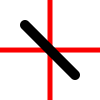
\includegraphics[width=1cm]{images/radicals/tu.png}& & & &\\ 
		enko & 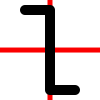
\includegraphics[width=1cm]{images/radicals/enko.png}& & & 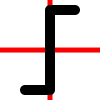
\includegraphics[width=1cm]{images/radicals/enkosewi.png} &\\ 
	\end{longtable}
\end{center}

\chapter{Cyrillic}
\begin{center}
    \begin{tabular}{l|c|c|c|c}
                  & Labial & Dental & Palatal & Velar \\
        \hline
		Nasal     &{\cf м} & {\cf н} &         &      \\
		Plosive   &{\cf п,б} & {\cf т,д}   &  &{\cf к,г}\\
		Fricative &        & {\cf с,з}    & {\cf ш}       &   {\cf х}   \\
		Affricate &        &  {\cf ц}     & {\cf ч}       & \\
		Tap       &        & {\cf р} & & \\
		Aprox.    & {\cf в} &  & {\cf ь/й} &
    \end{tabular}
\end{center}

Vowels are the standard Russian vowels. ``{\cf ь}'' is used after a consonant.

\begin{center}
	{\cf сан ареи ва кьен самаи та йору. кьо ва тинкури рисори цо кьенру. сан ареи ва тобаришухо сан масамаи ко.}
\end{center}
\chapter{Katakana}

\begin{center}
	\renewcommand{\arraystretch}{1.4}
	\begin{tabular}{c|ccccc}
		 & a & i & u & e & o \\ \hline
		 Ø & {\kf ア} & {\kf イ} & {\kf ウ} & {\kf エ} & {\kf オ} \\
		 k & {\kf カ} & {\kf キ} & {\kf ク} & {\kf ケ} & {\kf コ} \\
		 s & {\kf サ} & {\kf シ} & {\kf ス} & {\kf セ} & {\kf ソ} \\
		 t & {\kf タ} & {\kf チ} & {\kf ツ} & {\kf テ} & {\kf ト} \\
		 n & {\kf ナ} & {\kf ニ} & {\kf ヌ} & {\kf ネ} & {\kf ノ} \\
		 x & {\kf ハ} & {\kf ヒ} & {\kf フ} & {\kf ヘ} & {\kf ホ} \\
		 m & {\kf マ} & {\kf ミ} & {\kf ム} & {\kf メ} & {\kf モ} \\
		 j & {\kf ヤ} &  & {\kf ユ} &  & {\kf ヨ} \\
		 r & {\kf ラ} & {\kf リ} & {\kf ル} & {\kf レ} & {\kf ロ} \\
		 w & {\kf ワ} &  &  &  & {\kf ヲ} \\
		 n & {\kf ン} &  &  &  & 
	\end{tabular}
\end{center}

To create iotation or a syllable not present in Japanese, the small vowels ({\kf ァ ィ ェ ゥ ォ}) replace the previous vowel. Iotation is created with {\kf ィ} followed by another small another vowel.

{\kf サンアレイワケィエンサマイタヨロ.キィオワティンクリソツォサンアレイワトバリシゥホウセコ.}

\chapter{Devanagari}

\part{Texts}

\chapter{UDHR}
All human beings are born free and equal in dignity and rights. They are endowed with reason and conscience and should act towards one another in a spirit of brotherhood.

\begin{exe}
	\ex
	\gll osakota wa bu, kjo wa san kjo jo ta awuri ko. osa san are jo jo wa tinku isu co nu. are san jo wa suxo use ko. \\
		grouplead NOM COP.PRS.EV.0 3 NOM person 3 GEN ACC protect.INF DAT group people all GEN GEN NOM think conscience CONJ cop.PRS.EV.3 all person GEN NOM friend.IMP RECP DAT \\
	\trans `I believe governments exist to protect their people. I reason that all groups of people think and have conscience. All humans, be good to each other.'
\end{exe}

\chapter{I Lenin Takoj Molodoj}

\begin{tabular}{l|l}
	{\cf Неба утреннего стяг.}        & pjakaisu wa ru kikei noi te. \\
	{\cf В жизни важен первый шаг.}   & ču wa noxo iki te. \\ 
	{\cf Слышишь: реют над страною}   & ču wa ni ta jazucuruka: \\
	{\cf 	Ветры яростных атак!}     & ataki wa ru kikei te\\
	& \\
	{\cf 	припев:}                  & kire: \\ 
	{\cf 	И вновь продолжается бой,}  & jačo wa atakitu ni de.  \\
	{\cf 	И сердцу тревожно в груди.} & jačo wa ataki ta wiru.  \\
	{\cf 	И Ленин - такой молодой,}   & san Renin noreru ni de. \\
	{\cf 	И юный Октябрь впереди!}   & run ručii wa jačo ta weiru\\
	& \\		
	{\cf 	Весть летит во все концы:} & are wa ni ta sonaxaru. \\
	{\cf 	Вы поверьте нам, отцы, -}  & matja he wa jačo ta ronxo:\\
	{\cf 	Будут новые победы,}       & jani wa pobjerenju\\
	{\cf 	Встанут новые бойцы!}      & sanantaki wa renju\\
	& \\
	{\cf 	припев}                    & kire \\ 
	{\cf 	С неба милостей не жди!}   & pa wa maikuru kikei ci\\
	{\cf 	Жизнь для правды не щади.} & \\
	{\cf 	Нам, ребята, в этой жизни} & \\
	{\cf 	Только с правдой по пути!} & \\
	& \\
	{\cf 	припев}                    & kire \\ 
	{\cf 	В мире - зной и снегопад...} & \\
	{\cf 	Мир и беден и богат...} & \\
	{\cf 	С нами юность всей планеты -} & \\
	{\cf 	Наш всемирный стройотряд!} & \\
	{\cf 	припев}                  & kire \\ 
\end{tabular}

\chapter{pjukuxrepuno}

\begin{tabular}{l}
	pjuka ni wa sona osa Repuno jo ta jotu\\
	jaro činičikui te, san Čaku; san Kupai; ja co co 



\end{tabular}


\chapter{Quotes}

\section{Cat-v.org}

\begin{exe}
	\ex
	\gll ču wa ma ki jo ta masubu wo, ču wa ni ta čumaxaxo pjuka ču jo ci.\\ 
	2 ACC opposite thing GEN ACC disagree.PRS.SBJ CAUS 2 NOM DEM ACC leave.make.IMP documentation 2 GEN ABL.\\
	\trans `Don't include a sentence in documentation if its negation is obviously false.'
\end{exe}

\begin{exe}
	\ex 
	\gll ču wa ki ta sonadibu de, ču wa riso ni jo ta sonadixo \\
	2 NOM think ACC knowledge.give.PRS.SBJ TLOC, 2 NOM reason DEM GEN knowledge.give.IMP \\ 
	\trans `When explaining a command, or language feature, or hardware widget, first describe the problem it is designed to solve.'
\end{exe}


\chapter{Laws of Human Stupidity}
\part{Lexicon}
\chapter{Countries and Capitals}
\begin{center}
\begin{tabular}{l|c|c}
	English & Romanized & kijazu \\
	\hline
	Kievan Rus' & rusĭskaja zemlja  & Rusju \\
\end{tabular}
\end{center}

\begin{longtable}{lll}
	English & Romanized & Kijazu \\
	\hline
	Afghanistan &  &  \\
	Albania &  &  \\
	Algeria &  &  \\
	Andorra &  &  \\
	Angola &  &  \\
	Antigua and Barbuda &  &  \\
	Argentina &  &  \\
	Armenia &  &  \\
	Australia &  &  \\
	Austria &  &  \\
	Azerbaijan &  &  \\
	Bahamas &  &  \\
	Bahrain &  &  \\
	Bangladesh &  &  \\
	Barbados &  &  \\
	Belarus &  &  \\
	Belgium &  &  \\
	Belize &  &  \\
	Benin &  &  \\
	Bhutan &  &  \\
	Bolivia &  &  \\
	Bosnia and Herzegovina &  &  \\
	Botswana &  &  \\
	Brazil &  &  \\
	Brunei &  &  \\
	Bulgaria &  &  \\
	Burkina Faso &  &  \\
	Burundi &  &  \\
	Cambodia &  &  \\
	Cameroon &  &  \\
	Canada &  &  \\
	Cape Verde &  &  \\
	Central African Republic &  &  \\
	Chad &  &  \\
	Chile &  &  \\
	China &  &  \\
	Colombia &  &  \\
	Comoros &  &  \\
	Congo &  &  \\
	Costa Rica &  &  \\
	Croatia &  &  \\
	Cuba &  &  \\
	Cyprus &  &  \\
	Czech Republic &  &  \\
	Denmark &  &  \\
	Djibouti &  &  \\
	Dominica &  &  \\
	Dominican Republic &  &  \\
	Ecuador &  &  \\
	Egypt &  &  \\
	El Salvador &  &  \\
	Equatorial Guinea &  &  \\
	Eritrea &  &  \\
	Estonia &  &  \\
	Eswatini &  &  \\
	Ethiopia &  &  \\
	Fiji &  &  \\
	Finland &  &  \\
	France &  &  \\
	Gabon &  &  \\
	Gambia &  &  \\
	Georgia &  &  \\
	Germany &  &  \\
	Ghana &  &  \\
	Greece &  &  \\
	Grenada &  &  \\
	Guatemala &  &  \\
	Guinea &  &  \\
	Guinea-Bissau &  &  \\
	Guyana &  &  \\
	Haiti &  &  \\
	Honduras &  &  \\
	Hungary &  &  \\
	Iceland &  &  \\
	India &  &  \\
	Indonesia &  &  \\
	Iran &  &  \\
	Iraq &  &  \\
	Ireland &  &  \\
	Israel &  &  \\
	Italy &  &  \\
	Jamaica &  &  \\
	Japan &  &  \\
	Jordan &  &  \\
	Kazakhstan &  &  \\
	Kenya &  &  \\
	Kievan Rus' & rusĭskaja zemlja & rusju \\
	Kiribati &  &  \\
	Kuwait &  &  \\
	Kyrgyzstan &  &  \\
	Laos &  &  \\
	Latvia &  &  \\
	Lebanon &  &  \\
	Lesotho &  &  \\
	Liberia &  &  \\
	Libya &  &  \\
	Liechtenstein &  &  \\
	Lithuania &  &  \\
	Luxembourg &  &  \\
	Madagascar &  &  \\
	Malawi &  &  \\
	Malaysia &  &  \\
	Maldives &  &  \\
	Mali &  &  \\
	Malta &  &  \\
	Marshall Islands &  &  \\
	Mauritania &  &  \\
	Mauritius &  &  \\
	Mexico &  &  \\
	Micronesia &  &  \\
	Moldova &  &  \\
	Monaco &  &  \\
	Mongolia &  &  \\
	Montenegro &  &  \\
	Morocco &  &  \\
	Mozambique &  &  \\
	Myanmar &  &  \\
	Namibia &  &  \\
	Nauru &  &  \\
	Nepal &  &  \\
	Netherlands &  &  \\
	New Zealand &  &  \\
	Nicaragua &  &  \\
	Niger &  &  \\
	Nigeria &  &  \\
	North Korea &  &  \\
	North Macedonia &  &  \\
	Norway &  &  \\
	Oman &  &  \\
	Pakistan &  &  \\
	Palau &  &  \\
	Panama &  &  \\
	Papua New Guinea &  &  \\
	Paraguay &  &  \\
	Peru &  &  \\
	Philippines &  &  \\
	Poland &  &  \\
	Portugal &  &  \\
	Qatar &  &  \\
	Romania &  &  \\
	Russia &  &  \\
	Rwanda &  &  \\
	Saint Kitts and Nevis &  &  \\
	Saint Lucia &  &  \\
	%Saint Vincent and the Grenadines &  &  \\
	Samoa &  &  \\
	San Marino &  &  \\
	Sao Tome and Principe &  &  \\
	Saudi Arabia &  &  \\
	Senegal &  &  \\
	Serbia &  &  \\
	Seychelles &  &  \\
	Sierra Leone &  &  \\
	Singapore &  &  \\
	Slovakia &  &  \\
	Slovenia &  &  \\
	Solomon Islands &  &  \\
	Somalia &  &  \\
	South Africa &  &  \\
	South Korea &  &  \\
	South Sudan &  &  \\
	Spain &  &  \\
	Sri Lanka &  &  \\
	Sudan &  &  \\
	Suriname &  &  \\
	Sweden &  &  \\
	Switzerland &  &  \\
	Syria &  &  \\
	Taiwan &  &  \\
	Tajikistan &  &  \\
	Tanzania &  &  \\
	Thailand &  &  \\
	Timor-Leste &  &  \\
	Togo &  &  \\
	Tonga &  &  \\
	Trinidad and Tobago &  &  \\
	Tunisia &  &  \\
	Turkey &  &  \\
	Turkmenistan &  &  \\
	Tuvalu &  &  \\
	Uganda &  &  \\
	Ukraine &  &  \\
	United Arab Emirates &  &  \\
	United Kingdom &  &  \\
	United States &  &  \\
	Uruguay &  &  \\
	Uzbekistan &  &  \\
	Vanuatu &  &  \\
	Vatican City &  &  \\
	Venezuela &  &  \\
	Vietnam &  &  \\
	Yemen &  &  \\
	Zambia &  &  \\
	Zimbabwe &  &  \\

\end{longtable}

\chapter{Languages}
\chapter{Dates and Times}
\begin{center}
	\begin{tabular}{l|c|c}
		\textbf{English} & \textbf{Literal} & \textbf{Kijazu} \\
	\hline
	year    & orbit   & jutu \\ 
	month   & moon    & run \\
	week    & group   & osa \\
	day     & sun     & šiši\\
	hour    & section & se \\
	minute  & second section & se čii \\
	second  & heart   & lači \\  
\end{tabular}
\end{center}



\chapter{Linguistic Terminology}
\chapter{Computer Terminology}
\chapter{Mathematical Terminology}
\chapter{Science Terminology}
\printbibliography
\end{document}
